\chapter{Methods and data}

The following subsections provide a sufficient overview on the numerical model and analysis tools used for the presented work to allow a conclusive interpretation of the results thereafter.

\section{Region-Clustering} 
\label{sec:region_clustering}

\subsection{Regions \& Micro Regions}

Modern regional avalnche hazard assesment is based on several small \textit{micro-regiosn}, 
which are grouped during the process of the assesment in order to represent larger regions with similar conditions.
The pre-selections and definitions of those \textit{micro-regiosn} is crucial for a consitent assesment and
communication. The so called \textit{EUREGIO}, in especially the provinces of Tirol, South Tyrol and Trentino are 
currently divied into 37 sup-regions. A single forecasting region covers at least a area of 10x10 km.
The boundaries of these regions are typically along significant terrain signauters as mountain ridges or rivers.
The initial state of the \textit{micro-regiosn} are based on expert knowledge and where further adaped on 
expert feedback and further more on statitical analysis of meteorological data (Fig.: \ref{fig:EAWS_regions}).

\begin{figure*}[h]
    \centering
    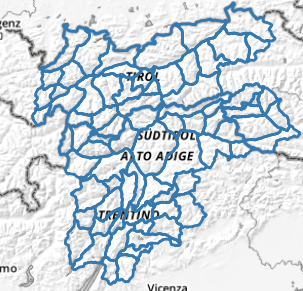
\includegraphics[width=0.5\textwidth]{Figures/figures_methods/micro_regions_EAWS.png}
    \caption{Outerlines of the EUREGIO micro-regions}
    \label{fig:EAWS_regions}
\end{figure*}

% ==== SNOWGRID ===============================================================
\subsection{SNOWGRID}
The \textit{SNOWGRID} model of the ZAMG ( Zentral Anstalft für Meteorologie und Geodynamik)
 is a combination of the nocasting-system INCA and radiation model \textit{STRAHLGRID}. INCA delivers forecasts for
 temperature, precipitation, wind and clouds. INCA has a spatial resolution of 1x1km further more with a topogrphical
 downscaling of 100x100m. \textit{SNOWGRID} calculates on the basis auf INCA solid precipitation
 and analyses changes from the past 3 days. Furthermore \textit{SNOWGRID} takes the heat content and the settling of 
 the snowpack and the sinking effect of snowline in valleys into account. It delivers the information of the total
 snowhight in a spatial resolution of 100x100m in 15 min interval.(Fig.: \ref{fig:snowgrid})

 \begin{figure*}[h]
    \centering
    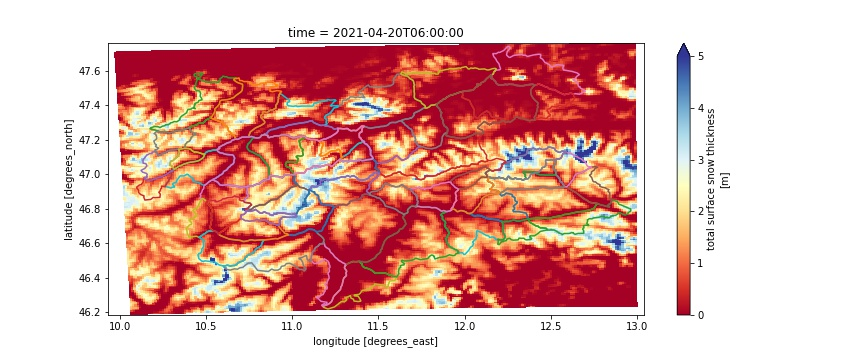
\includegraphics[width=0.8\textwidth]{Figures/figures_methods/snowgrid.jpg}
    \caption{Total snowhight of the SNOWGRID model for the 1st March 2021 06:00:00 MEZ}
    \label{fig:snowgrid}
\end{figure*}

\noindent In order to validate the Regions relevant for avalanche warning service EUREGIO only the wintermonths from Oct till March 
over the periods of the past 10 years (November 2011 till March 2021) comes into account. In the scope of a saveing computing 
power the spatial resolution of 100x100m is reduced to 1x1km by taking the median within this spector. 
Based on the 06:00:00MEZ datastamp a 24h surface hight change will be calulated.

% ==== Cost733cat ===============================================================

\subsection{Cost733cat - Weather and circulation type classification}

The Cost733cat is a databease of weather and circulation type classfication covering a spatial domain over Europe with 
12 sup domains of the ZAMG. The inputdata comes from ERA40-reanalysis dataset provided by the Eruopian Center of Medium-Range
Weather forecast by \textcite{philippCost733catDatabaseWeather2010}. The domain of intresst of this research is D06 covering
the alps. 

\noindent The Cost733cat contains informations about the main wind direction, cyclonisity and humidity on different pressure levels
weighted to the center of the domain. For these research only the information about the main flow at 700 hPa is of intresst.
The main flow is devided into 9 windsectors, 4 main wind sectors, 4 side wind sectors and one additional class for changing 
wind regimes within a day. For further statistical analyis it has to be taken into account that main sectors has a coverage of
30 $^{\circ}$ and side sectors 60 $^{\circ}$:
\\

\begin{minipage}{.5\linewidth}
    \begin{itemize}
        \item 345$^{\circ}$ -   15$^{\circ}$  \dots   N
        \item 15$^{\circ}$  -   75$^{\circ}$    \dots NE
        \item 75$^{\circ}$  -   105$^{\circ}$    \dots E
        \item 105$^{\circ}$  -   165$^{\circ}$    \dots SE
        \item 165$^{\circ}$  -   195$^{\circ}$    \dots S
        \item 195$^{\circ}$  -   255$^{\circ}$    \dots SW
        \item 255$^{\circ}$  -   285$^{\circ}$    \dots W
        \item 285$^{\circ}$  -   345$^{\circ}$    \dots W
    \end{itemize}
    \end{minipage}
    \hfill
    \begin{minipage}{.5\linewidth}
    \centering
    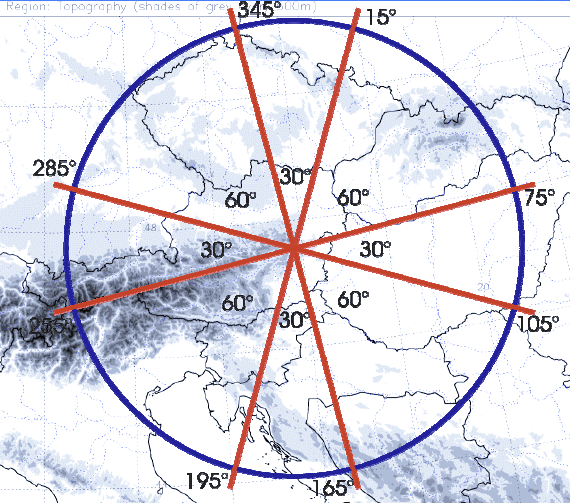
\includegraphics[width=\linewidth]{Figures/figures_methods/windesctors.png}
    \captionof{figure}{Windsectors of the Cost733cat \textcite{krennertWetterlagenklassifikationenZAMGAnfangen}}
    \end{minipage}

% ==== Clustering ===============================================================

\subsection{Clustering}


% ==== Assesing Avlanche Problems ===============================================================
\subsection{Assesing Avlanche Problems}


% ==== SNOWPACK ===============================================================
\subsection{SNOWPACK}


% ==== Avalanche Problems ===============================================================
\subsection{Avalanche Problems}


% ==== Avalnche Problem Algorithm ===============================================================
\subsection{Avalnche Problem Algorithm}

 %\begin{figure*}[tbp]
%     \centering
%     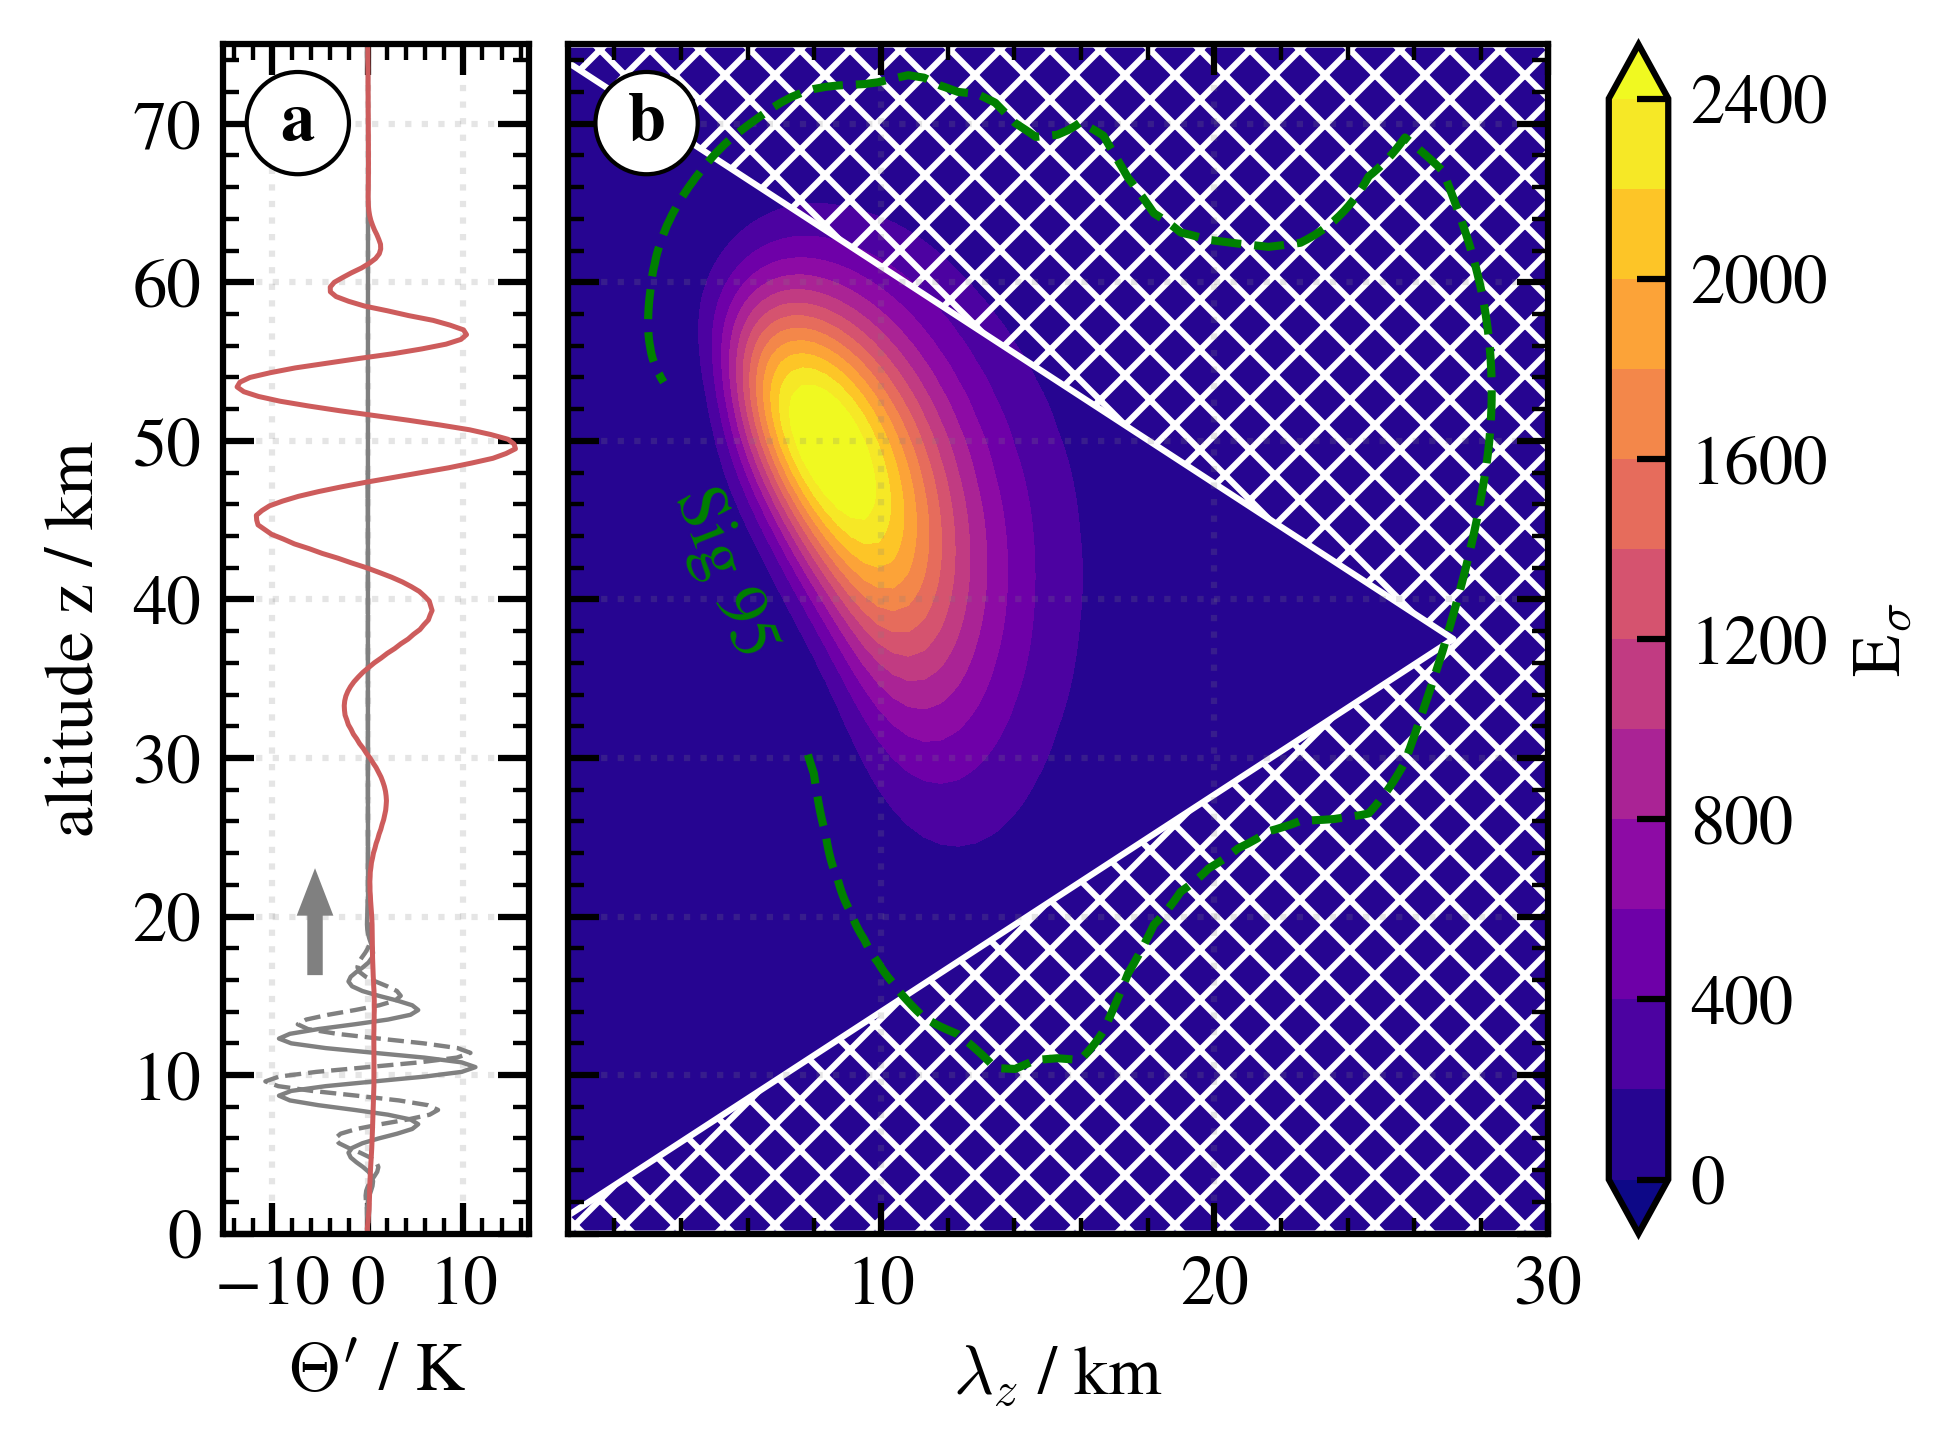
\includegraphics[width=0.99\textwidth]{figures_methods/waveletAna_power_spectrum.png}
%     \caption{}
%     \label{fig:wavelet_example}
% \end{figure*}
